\documentclass[final]{beamer}
\mode<presentation>
  {
  \usetheme{Rutgers}
  }
  \usepackage{amsmath,amsthm, amssymb, latexsym}
  \boldmath
  \usepackage[english]{babel}
  \usepackage[latin1]{inputenc}
  \usepackage{lmodern}
  \usepackage[orientation=portrait,size=a0,scale=1.4,debug]{beamerposter}
  
\usepackage{myalgorithm}
\usepackage{wrapfig}
\usepackage[noend]{myalgorithmic}
\usepackage{multirow}
\usepackage{multicol}
\usepackage{graphicx,wrapfig,lipsum}


  %%%%%%%%%%%%%%%%%%%%%%%%%%%%%%%%%%%%%%%%%%%%%%%%%%%%%%%%%%%%%%%%%%%%%%%%%%%%%%%%%
  \title[Maneuvers]{Learning Efficient Maneuver Sets for Kinodynamic Motion Planning}
  \author[Sivaramakrishnan]{Aravind Sivaramakrishnan, Zakary Littlefield and Kostas E. Bekris}
  \institute[Rutgers]{Department of Computer Science, Rutgers, the State University of New Jersey}



  %%%%%%%%%%%%%%%%%%%%%%%%%%%%%%%%%%%%%%%%%%%%%%%%%%%%%%%%%%%%%%%%%%%%%%%%%%%%%%%%%
  \newlength{\blocklen}
  \begin{document}
  \setlength{\blocklen}{0.49\textwidth}
  \begin{frame}[t]{} 
    \vspace {-0.5in}
    \begin{columns}[t]
	\begin{column}{0.50\textwidth}
		\begin{block}{\large Motivation}
		    \centering
		    % \begin{columns}[t]
			   %  \begin{column}{0.97\textwidth}
				    \vspace{-0.1in}
				    \begin{itemize}
					    \item Provide a dataset for the task of robotic grasping and manipulation in a \\typical constrained warehouse environment
					    \item A difficult environment:
					   	\begin{itemize}
					   		\item Inconsistent and indirect lighting conditions induce noise in sensors 
					   		\item Objects are often partially occluded by other objects or the shelving unit
					   		\item Narrow bins allow only very limited robotic mobility 
					   	\end{itemize}
					   	\item However, the task is of great importance to industrial applications 
					   	\item Developing high accuracy pose estimation algorithms is of utmost importance
					   	\item \textbf{Objective:} provide a representative dataset that \emph{allows researchers to \\determine effects of specific environmental variables on pose estimation algorithms} 
				    \end{itemize}
			   %  \end{column}
		    % \end{columns}
		\end{block}
	\end{column}
	\begin{column}{0.50\textwidth}
		\begin{block}{\large Amazon Picking Challenge (APC)}
		    \centering
		    	\begin{figure}[h]
		    		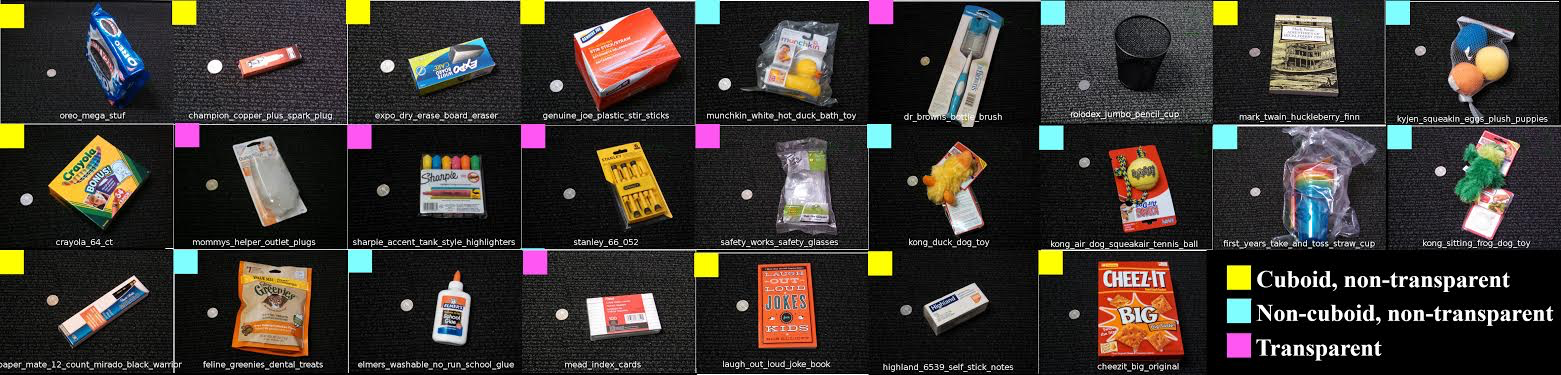
\includegraphics[width = 0.75\textwidth, height=2.5in]{meta_items}	\hspace{0.1in}
		    		\caption{The 25 APC objects categorized by broad object class}
	    		\end{figure}
	    		\vspace{-0.2in}
		    \begin{columns}[T]
		    	\begin{column}{0.98\textwidth}
					\begin{itemize}
						\item Shelf-picking challenge simulating a warehouse environment
						\item Tight, cluttered workspaces bins within the shelving unit
						\item 25 target objects stocked in 12 bins, 1-4 objects per bin
						\item Target items show variety of forms and traits
					\end{itemize}
				\end{column}
				% \begin{column}{0.38\textwidth}
				% 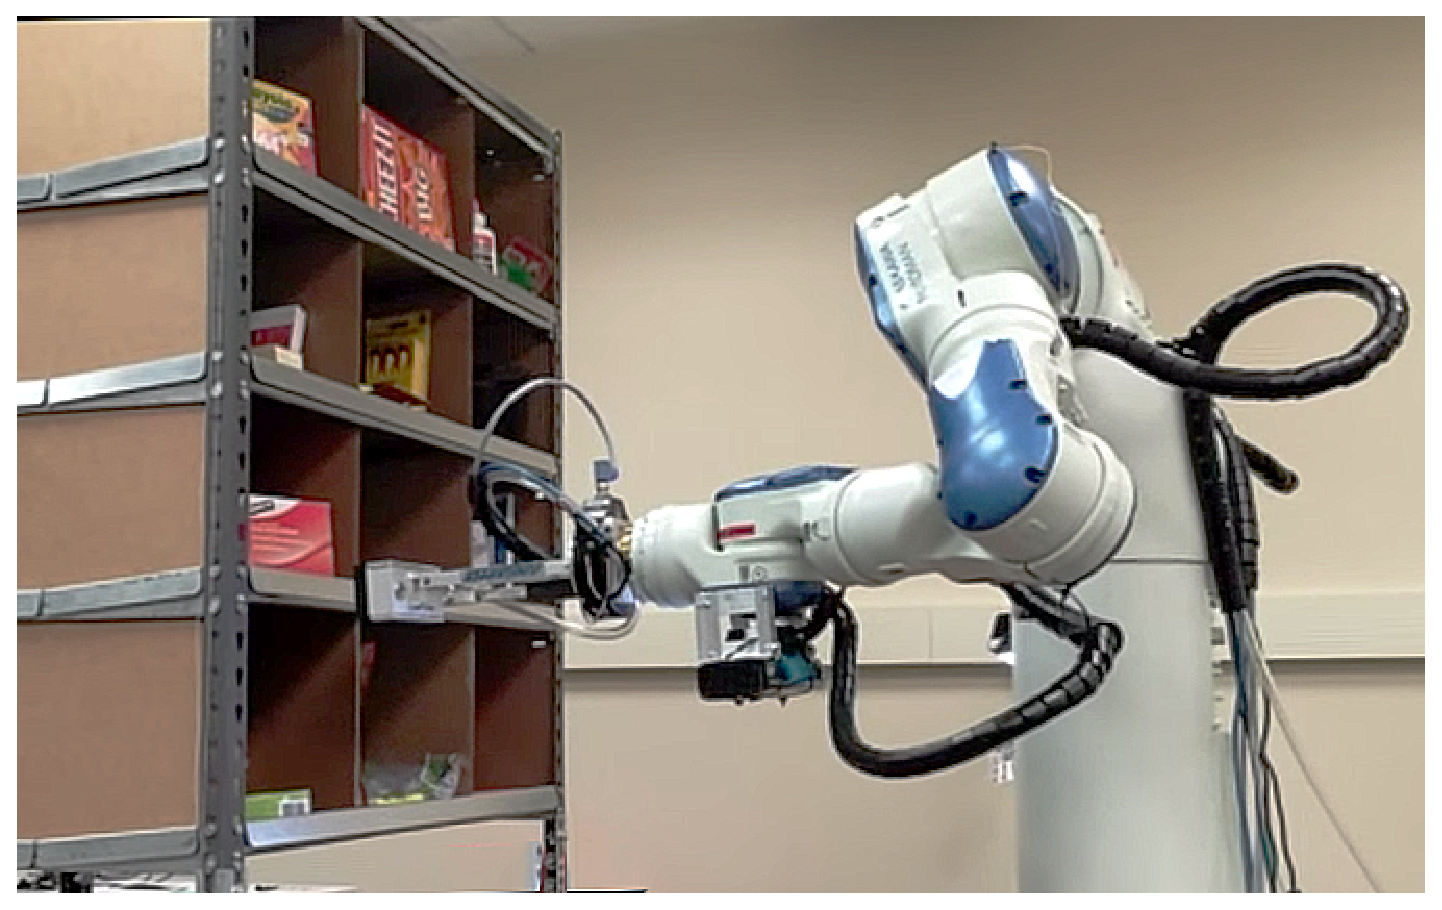
\includegraphics[height=2.5in]{datacollectionsetup_2}	\hspace{0.1in}
				% \end{column}
			\end{columns}
		\end{block}
	\end{column}
\end{columns}	
		    

    \vfill
    
\begin{columns}[t]
	\begin{column}{0.65\textwidth}
		\begin{block} {\large Input to the learning process}
			\begin{columns}[T]
				\centering
				\begin{column}{0.59\textwidth}
					\begin{itemize}
						\item A regular set of points $\mathbb{X}_{local}$ in the vicinity of $x_0$ are collision checked to generate a binary 2D map $o_{local}$ indicating the presence of obstacles in the workspace.
						\item The heuristic $h(x)$ is also evaluated at each $x \in \mathbb{X}_{local}$, resulting in a 2D matrix $h_{local}$.
					\end{itemize}
				\end{column}
				\begin{column}{0.20\textwidth}
					\centering
					\begin{figure}
					
\includegraphics[width=0.5\columnwidth]{o_example}
					\caption{$o_{local}$} 
					\end{figure}
				\end{column}
				\begin{column}{0.20\textwidth}
					\centering
					\begin{figure}
					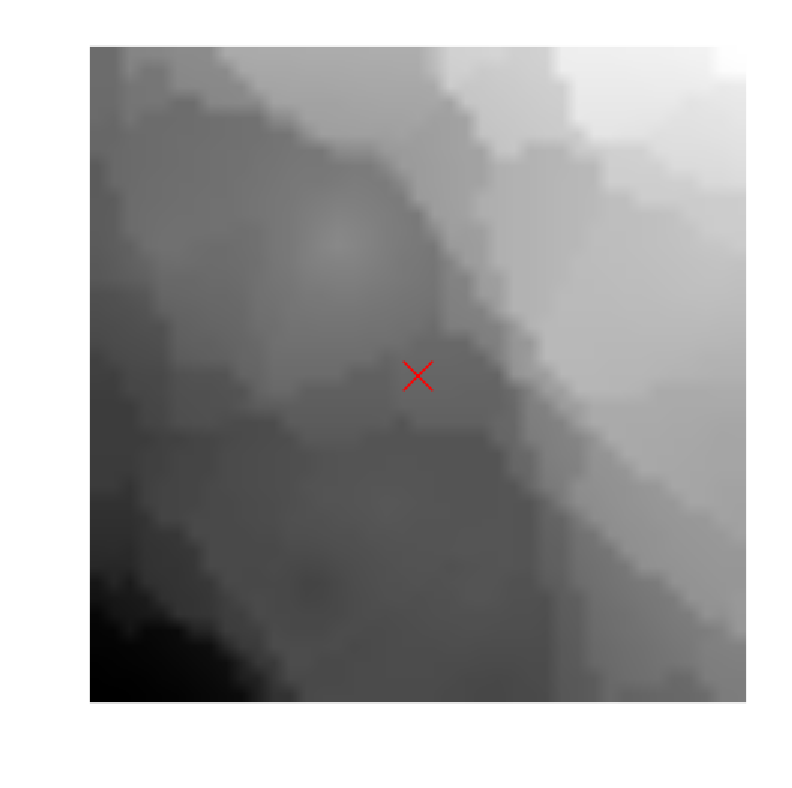
\includegraphics[width=0.5\columnwidth]{h_example}
					\caption{$h_{local}$} 
					\end{figure}
					\vspace{0.1in}
				\end{column}
			\end{columns}
		\vspace{-0.4in}
		\end{block}
		\begin{block}{\large Proposed architecture}
			\begin{itemize}
			\item Multi-layered neural networks $F_x, F_o, F_h$ act on the inputs to produce $x_0^*, o_{local}^*, h_{local}^*$. 
			\item An operator $M_0(x_0^*, o_{local}^*,h_{local}^*)$ produces feature vector  $x_f^0$.
			\item Exploitative control $u^0$ is obtained as $u^0 = F^0(x_f^0)$, where $F^0$ is also a neural network.
			\item Remaining $N$ exploratory controls are obtained as follows.
			\vspace{-.1in}
			\begin{align*}
				x_f^k &= M_k(x_f^0,U_{k-1}) \\
				u^{k} &= F^k(x_f^k) 
			\end{align*}
			\vspace{-.1in}
			where for all $k \geq 1$, $U_k = \{u^0,u^1,..,u^{k-1}\}$. For the exploitative control ($k=0$), $U_{k-1}$ is the empty set.
			\vspace{0.1in}
			\end{itemize}			
			\begin{figure}[h!]
				\centering
				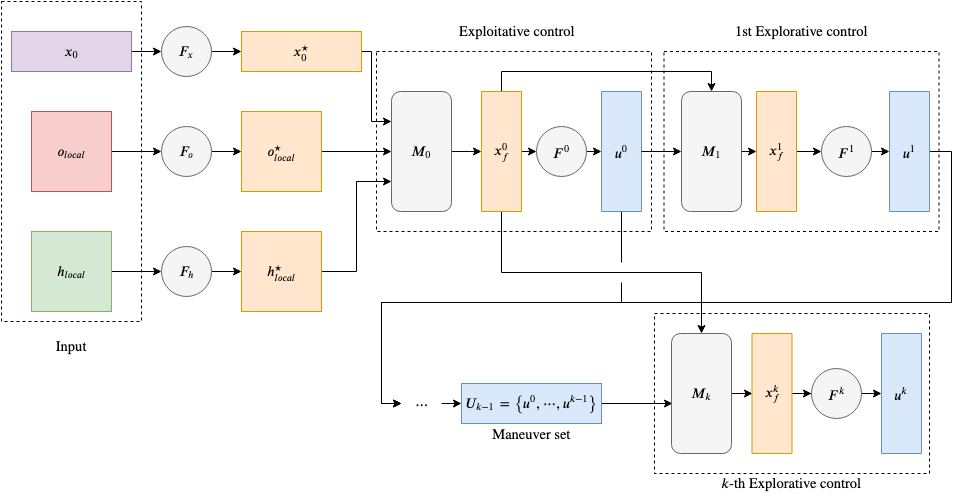
\includegraphics[scale=0.95]{cgraph}
				\vspace{-.1in}
				\caption{Computation graph of $U_k = \hat{f}(x_0,o_{local},h_{local})$. For $k=N, U_k = \hat{U} = \{u^0,\cdots,u^N\}$.\vspace{-.15in}}
				\label{fig:cgraph}
			\end{figure}
			\vspace{-.1in}
		\end{block}
	\end{column}
	\begin{column} {0.35\textwidth}
		\begin{block}{\large Experimental Setup}
		\begin{figure}[h!]
			\centering
			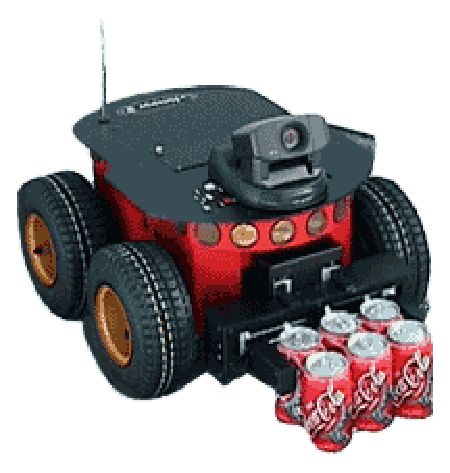
\includegraphics[scale=0.75]{skid-steer}
			\vspace{-.1in}
			\caption{Treaded vehicle with 5 dim. state space (SE(2) augmented by steering angle and forward velocity) and 2 dim. control space (acceleration of left and right treads) used in our experiments.}
		\end{figure}
		\begin{itemize}
			\item Randomly place obstacles in the workspace so they cover one-third of the reachable workspace. 
			\item Execute the DIRT planner $[1]$ with the online curation procedure on multiple problem instances in such workspaces. 
			\item Euclidean distance to the goal in the workspace is used as the heuristic function. %The cost is the duration of the solution trajectory.
			\item For each node $x_0$ the planner selects to propagate, store $o_{local}$ and $h_{local}$ maps, and maneuver set $\hat{U}$ of size 5 curated from 1000 randomly sampled maneuvers.
			\item Train two networks - fully connected (\texttt{FC}) and convolutional (\texttt{Conv})
		\end{itemize}
		\centering
			\vspace{0.2in}
			\begin{columns}
				\centering
				\begin{column}{0.4\columnwidth} 
					\centering
					\begin{figure}
					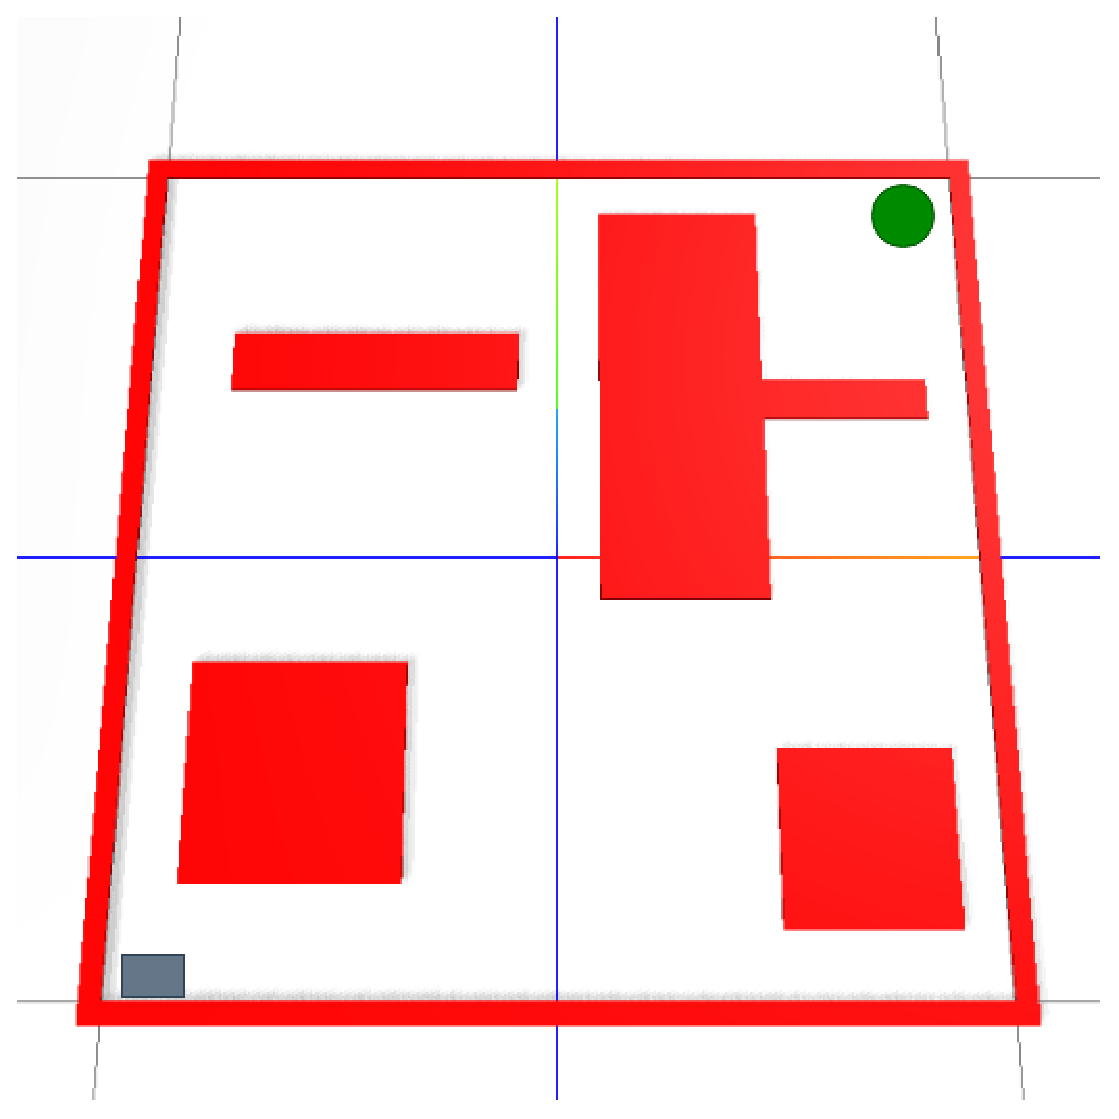
\includegraphics[scale=0.5]{iai}
					\caption{\texttt{Greedy}} 
					\end{figure}
				\end{column}
				\hfill
				\begin{column}{0.4\columnwidth} 
					\centering
					\begin{figure}
					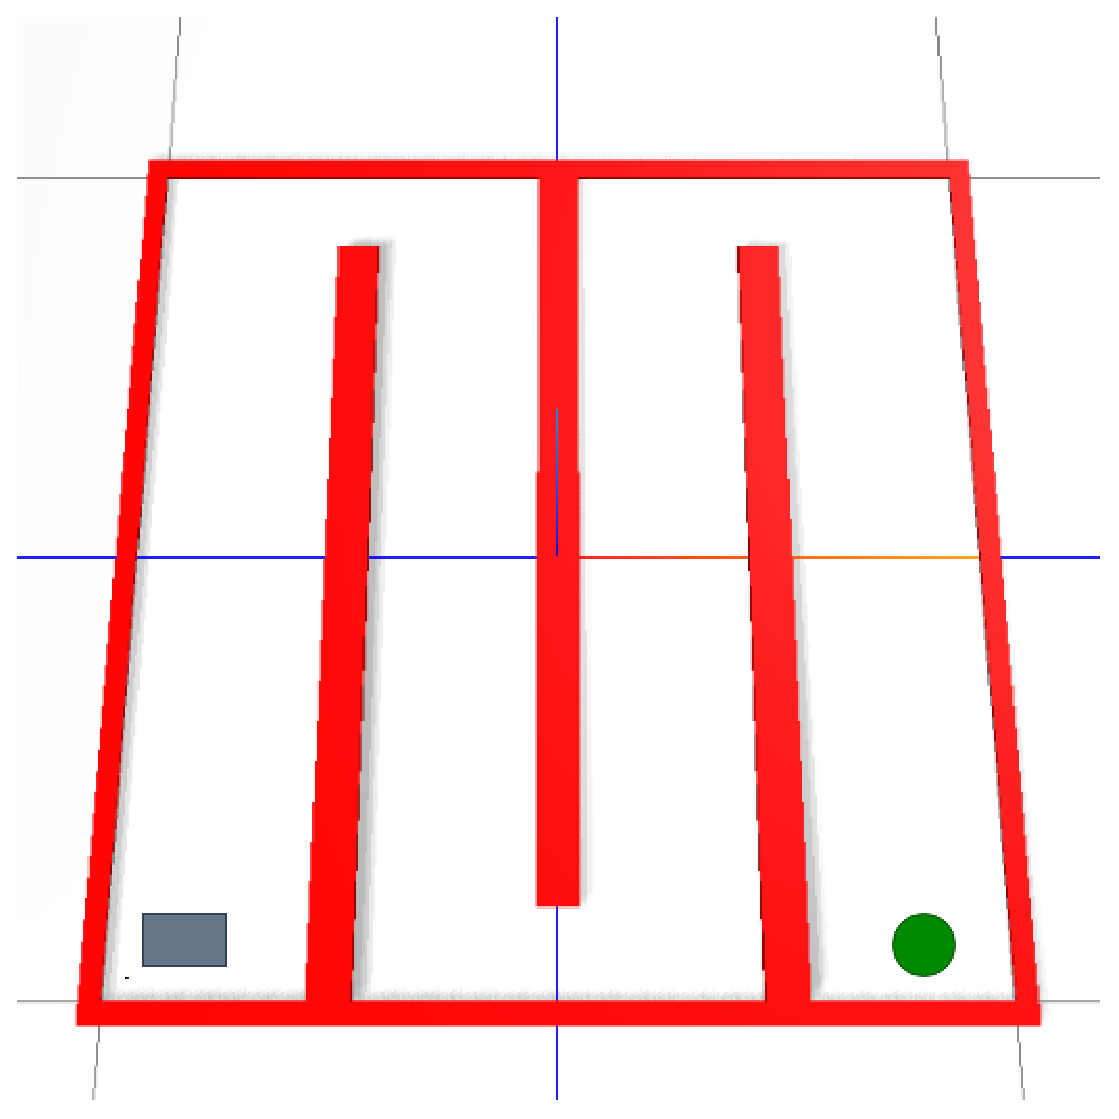
\includegraphics[scale=0.5]{flappy}
					\caption{\texttt{Explore}} 
					\end{figure}
				\end{column}
			\end{columns}
			\vspace{0.2in}
			\small{Environments: The grey rectangle is the starting pose of the robot (facing right) and the green circle is the goal region. The robot must avoid the red obstacles.}
			\vspace{0.1in}
		\end{block}
	\end{column}
\end{columns}




    \vfill
    \begin{columns}[t]
	\begin{column}{0.32\textwidth}
		\begin{block}{\large Pose Estimation Evaluation}
			\centering
			\begin{itemize}
				\item Dataset is readily used to compare pose estimation algorithms for this difficult task 
				\item Acceptable accuracy thresholds are at the discretion of the user
				\item May use the metrics provided by the dataset to determine a series of improvements in order to deal with difficulties of the task
			\end{itemize}
				\begin{figure}[h]
					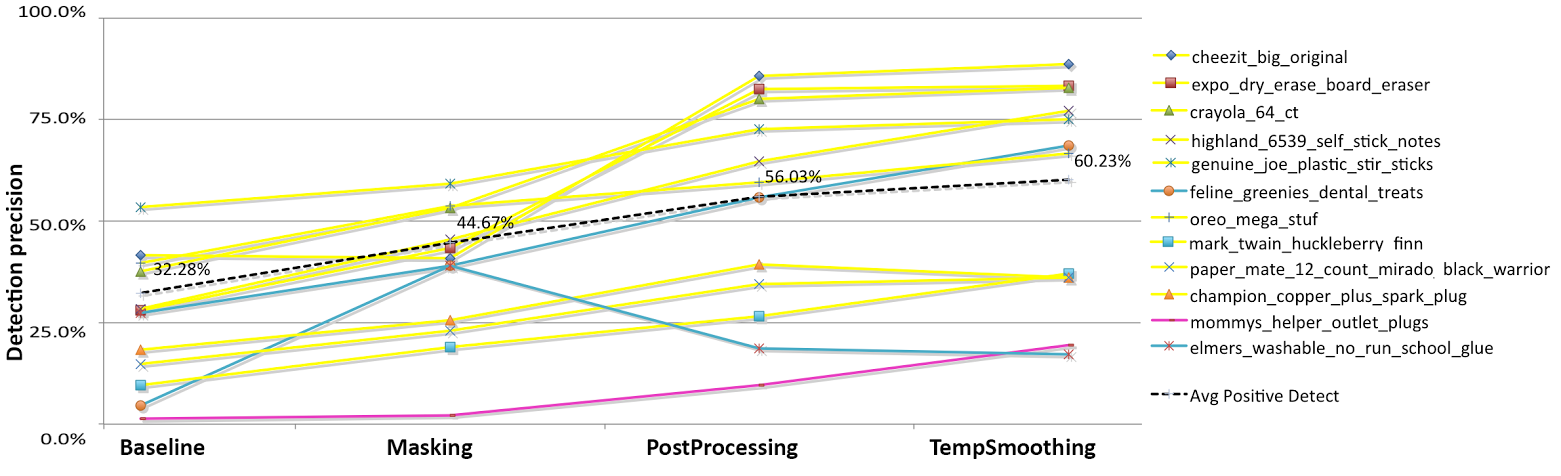
\includegraphics[width = 0.9\textwidth]{results}
					\caption{Evaluation made possible several improvements to an example pose estimation algorithm }
				\end{figure}
				\begin{figure}[h]
					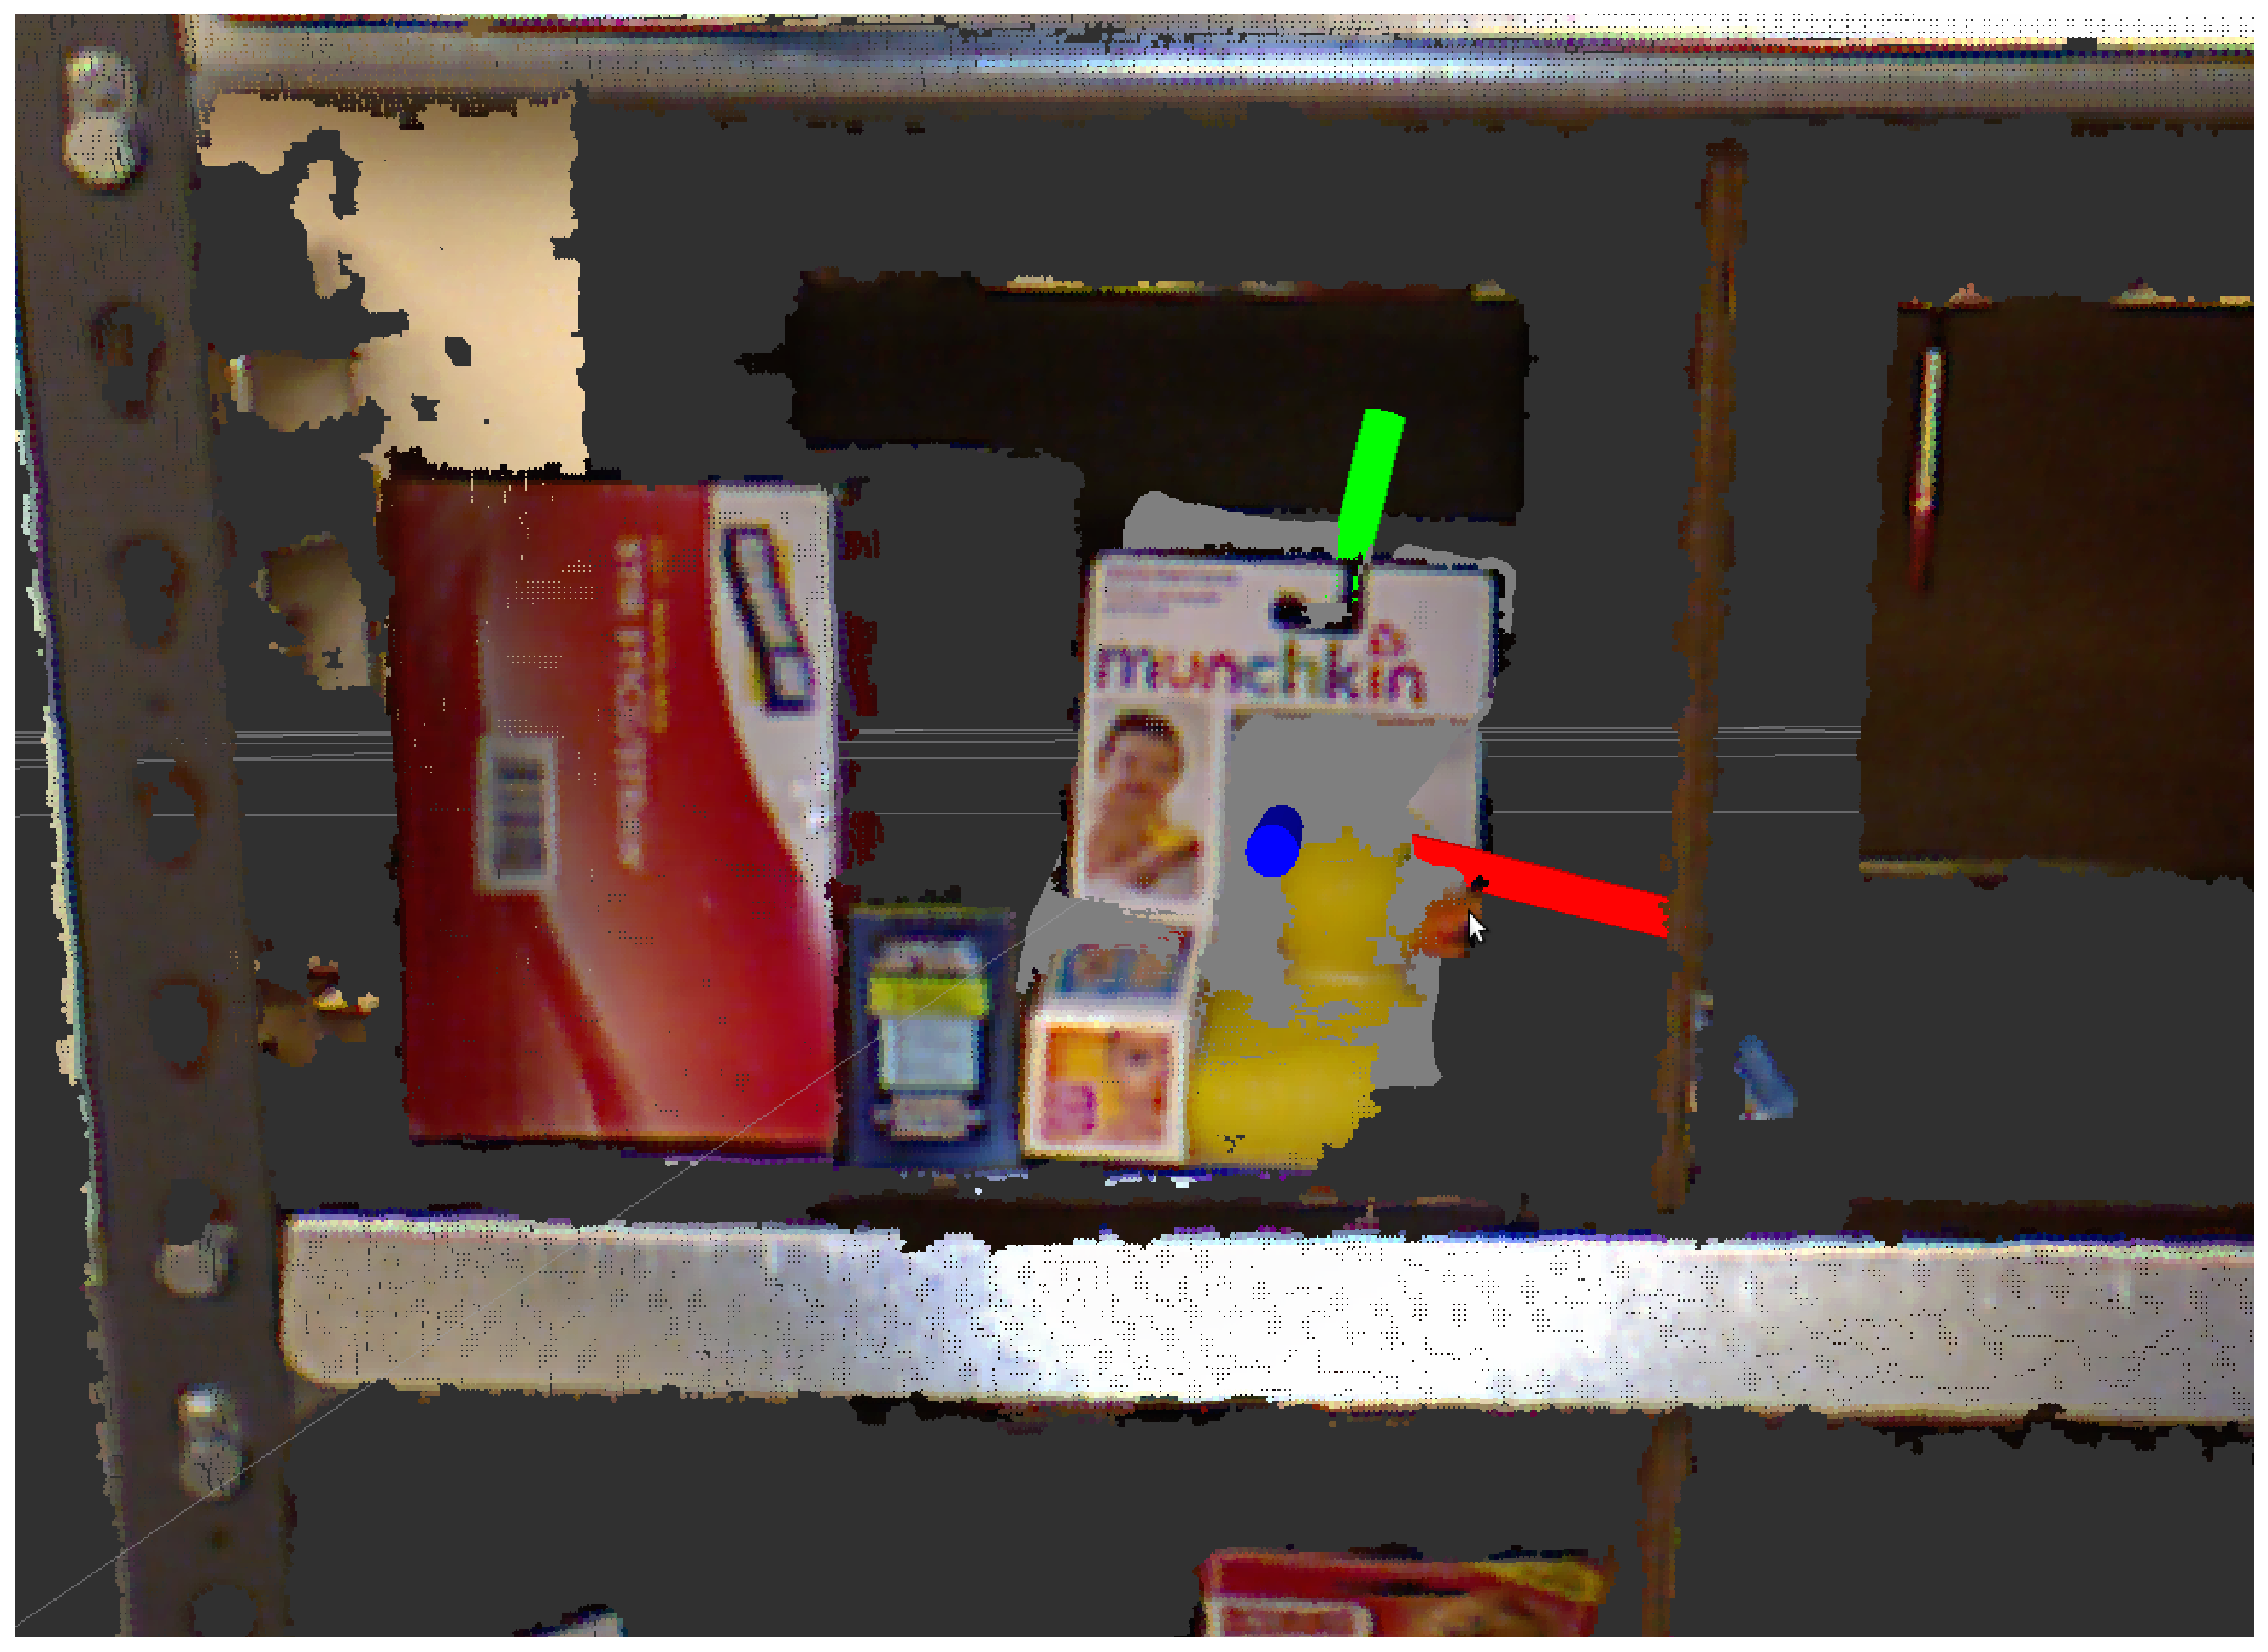
\includegraphics[width = 0.7\textwidth]{munchkin_det}
					\caption {An example detection of the ``duck'' from our dataset}
				\end{figure}
		\end{block}
	\end{column}
	\begin{column}{0.68\textwidth}
		\begin{block}{\large Dataset Comparison}
			\centering
			\vspace{-0.2in}
				\begin{figure}[h]
					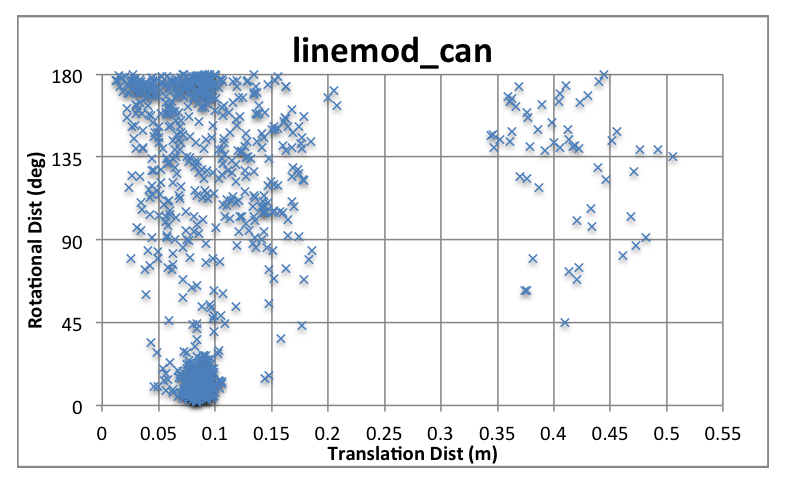
\includegraphics[width = 0.3\textwidth]{linemod_can_results}
					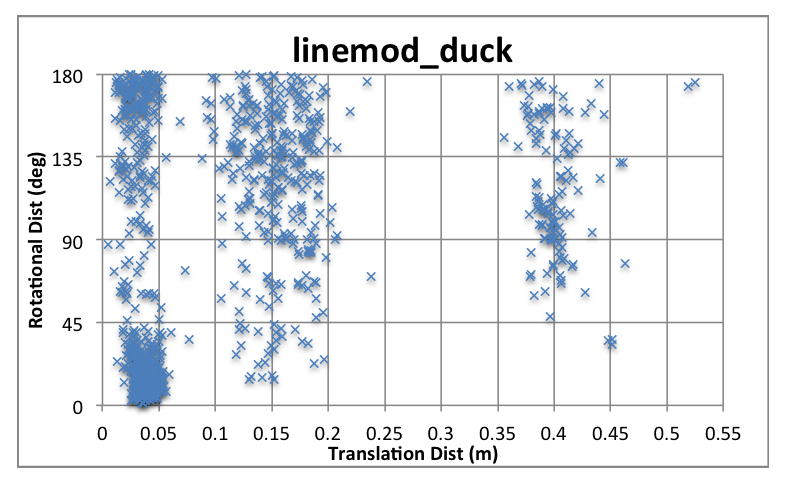
\includegraphics[width = 0.3\textwidth]{linemod_duck_results}
					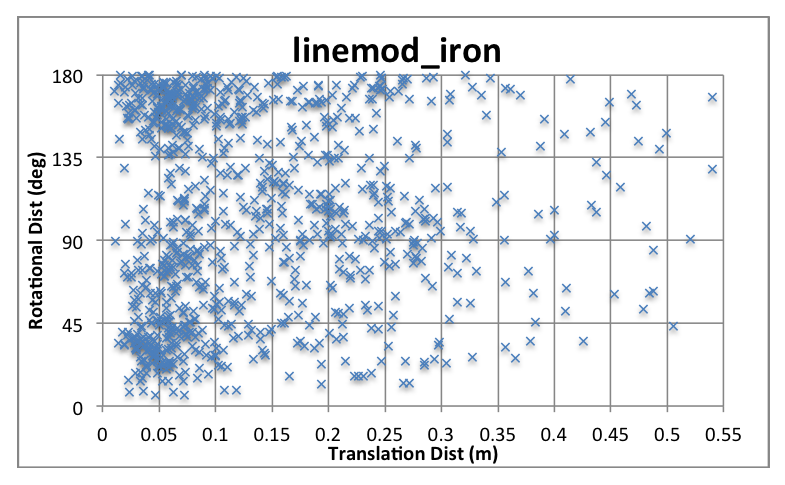
\includegraphics[width = 0.3\textwidth]{linemod_iron_results}
					\vspace{-0.2in}
					\caption{Example objects from LINEMOD dataset evaluated using our example algorithm}
				\end{figure}
			\vspace{-0.2in}
			\begin{itemize}
				\item LINEMOD dataset of 10,000+ RGBD images with ground truth 6D pose
				\item Shows target items on an AR board, in a heavily cluttered environment
				\item Samples generated from a variety of viewpoints around and above the object
				\item Can evaluate rotational, translational accuracy using the provided object models 
			\end{itemize}
				\begin{figure}[h]
					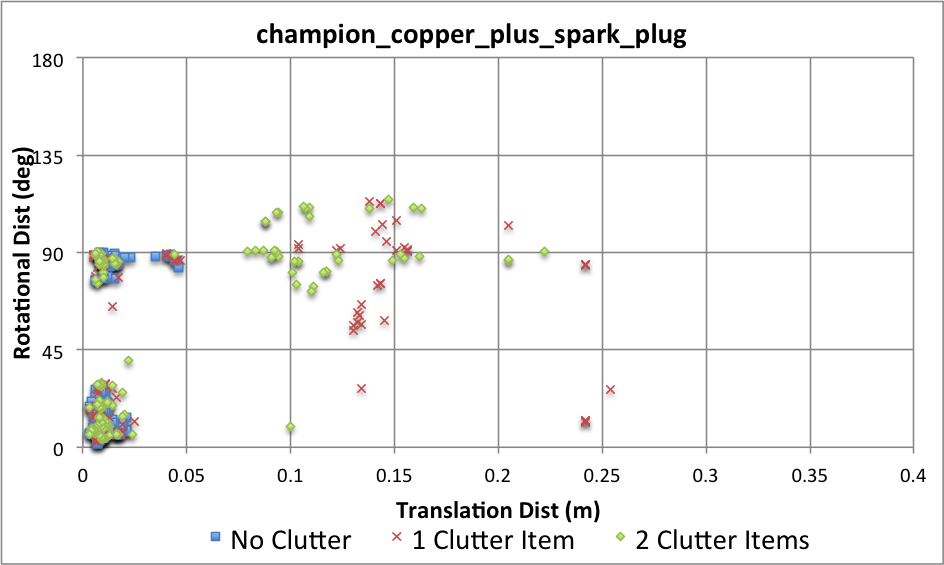
\includegraphics[width = 0.3\textwidth]{scatter_champion}
					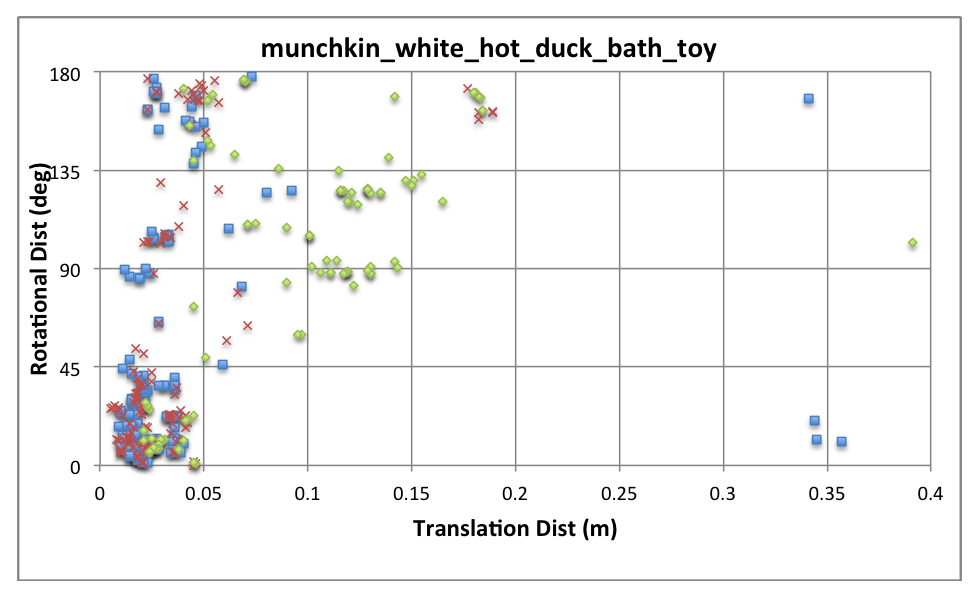
\includegraphics[width = 0.3\textwidth]{scatter_munchkin}
					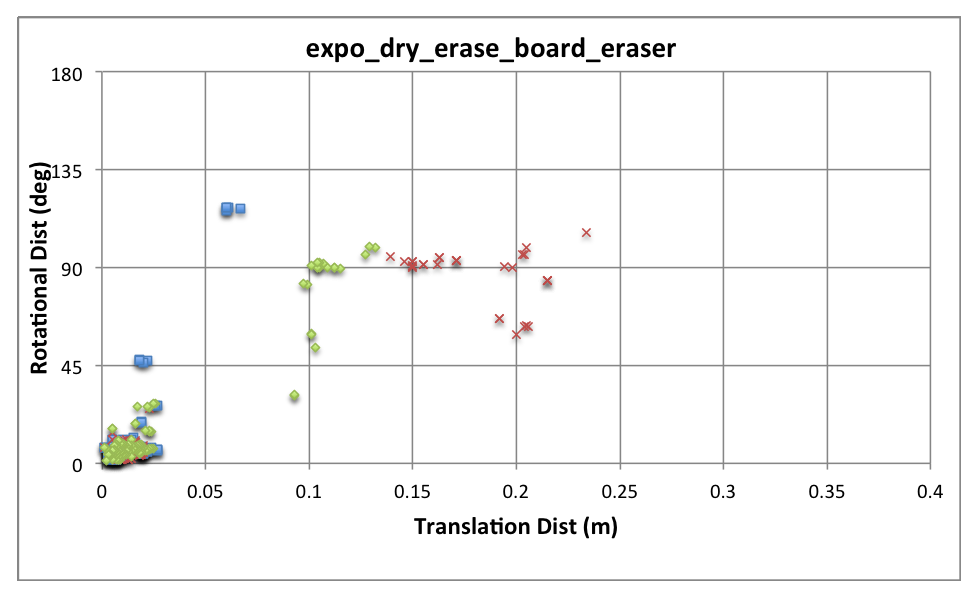
\includegraphics[width = 0.3\textwidth]{scatter_expo}
					\vspace{-0.2in}
					\caption{Objects from our dataset evaluated using the same algorithm; Colors indicate clutter conditions}
				\end{figure}
			\vspace{-0.2in}
			\begin{itemize}
				\item Our similar setup: object models provided, 10,000+ RGBD images
				\item Able to extract effects of immediate clutter on accuracy
				\item Can also determine robustness to noise in the sensor samples
				\item Evaluation with our dataset allows researchers to identify certain weak points in pose estimation algorithms on this difficult task
			\end{itemize}
		\end{block}
	\end{column}
\end{columns}
    \vfill
    \bibliographystyle{IEEEtran}
    \bibliography{PlanRob.bib}
  \end{frame}
\end{document}


%%%%%%%%%%%%%%%%%%%%%%%%%%%%%%%%%%%%%%%%%%%%%%%%%%%%%%%%%%%%%%%%%%%%%%%%%%%%%%%%%%%%%%%%%%%%%%%%%%%%
%%% Local Variables: 
%%% mode: latex
%%% TeX-PDF-mode: t
%%% End:
